% Paquets généraux
\documentclass[a4paper,12pt,titlepage]{article}
\usepackage[T1]{fontenc}
\usepackage[utf8]{inputenc}
\usepackage[french]{babel}
\usepackage[gen]{eurosym}
%\usepackage[dvips]{graphicx}
\usepackage{fancyhdr}
\usepackage{pdfpages} 
\usepackage{multido}
\usepackage{hyperref}
%\usepackage{textcomp}
%\usepackage{aeguill}
\usepackage{schemabloc}
\usepackage[bitstream-charter]{mathdesign}

\newcommand{\id}{54}
\newcommand{\nom}{Liaisons mécaniques}
\newcommand{\sequence}{04}
\newcommand{\num}{01}
\newcommand{\type}{TP}
\newcommand{\descrip}{Modélisation d'un solide. Comportement des liaisons mécaniques. Modéliser les mécanismes du laboratoire par un schéma cinématique, paramétré.}
\newcommand{\competences}{A3-C4: Analyse d'architecture et de comportement \\ &  Mod1-C1: Isolement d'un solide ou d'un système de solides \\ &  Mod2-C10-1: Modèle de solide indéformable \\ &  Mod2-C11: Modélisation géométrique et cinématique des mouvements entre solides indéformables \\ &  Mod2-C12: Modélisation cinématique des liaisons entre solides \\ &  Mod2-C15: Modélisation des actions mécaniques \\ &  Rés-C6: Utilisation d'un solveur ou d'un logiciel multi physique \\ &  Com1-C1: Différents descripteurs introduits dans le programme \\ &  Com2-C4: Outils de communication}
\newcommand{\nbcomp}{9}
\newcommand{\systemes}{Plateforme Stewart}
\newcommand{\systemessansaccent}{Plateforme Stewart}
\newcommand{\ilot}{2}
\newcommand{\ilotstr}{02}
\newcommand{\dossierilot}{\detokenize{Ilot_02 Plateforme Stewart}}
\newcommand{\imageun}{Plateforme}

\newcommand{\urlsysteme}{\href{https://www.costadoat.fr/systeme/57}{Ressources système}}
\newcommand{\matlabsimscape}{\href{https://github.com/Costadoat/Sciences-Ingenieur/raw/master/Systemes/Plateforme Stewart/Plateforme_Stewart_Simscape.zip}{Modèle Simscape}}
\newcommand{\solidworks}{\href{https://github.com/Costadoat/Sciences-Ingenieur/raw/master/Systemes/Plateforme Stewart/Plateforme_Stewart_Solidworks.zip}{Modèle Solidworks}}
\newcommand{\edrawings}{\href{https://github.com/Costadoat/Sciences-Ingenieur/raw/master/Systemes/Plateforme Stewart/Plateforme_Stewart.EASM}{Modèle eDrawings}}
\newcommand{\test}{Stewart_param1}
\newcommand{\testi}{Stewart_param2}
\newcommand{\testii}{Stewart_param3}
\newcommand{\testiii}{Stewart_param4}
\newcommand{\testiiii}{Stewart_euler}

\newcommand{\auteurun}{Renaud Costadoat}
\newcommand{\auteurdeux}{Françoise Puig}
\newcommand{\institute}{Lycée Dorian}


\usepackage{color}
\usepackage{xcolor}
\usepackage{colortbl}
\usepackage{helvet}
\renewcommand{\familydefault}{\sfdefault}
\usepackage{amsfonts}
\usepackage{amsmath}
%\usepackage{xspace}
\usepackage{varioref}
\usepackage{tabularx}
%\usepackage{floatflt}
\usepackage{graphics}
\usepackage{wrapfig}
\usepackage{textcomp}
\usepackage{tikz}
\usepackage{wrapfig}
\usepackage{gensymb}
\usepackage[european]{circuitikz}
\usetikzlibrary{babel}
\usepackage{ifthen}
\usepackage{cancel}
\usepackage{etoolbox}
\usepackage{multirow}
%\usepackage{boxedminipage}
\definecolor{gris25}{gray}{0.75}
\definecolor{bleu}{RGB}{18,33,98}
\definecolor{bleuf}{RGB}{42,94,171}
\definecolor{bleuc}{RGB}{231,239,247}
\definecolor{rougef}{RGB}{185,18,27}
\definecolor{rougec}{RGB}{255,188,204}%255,230,231
\definecolor{vertf}{RGB}{103,126,82}
\definecolor{vertc}{RGB}{220,255,191}
\definecolor{forestgreen}{rgb}{0.13,0.54,0.13}
\definecolor{blcr}{rgb}{0.59,0.69,0.84}
\definecolor{blfr}{rgb}{0.32,0.51,0.75}
\definecolor{orfr}{rgb}{0.90,0.42,0.15}
\definecolor{orcr}{rgb}{0.90,0.65,0.50}
\definecolor{orangef}{rgb}{0.659,0.269,0.072}
\definecolor{orange}{rgb}{0.58,0.35,0.063}
\definecolor{orangec}{rgb}{0.43,0.32,0.25}
\definecolor{rcorrect}{rgb}{0.6,0,0}
\definecolor{sequence}{rgb}{0.75,0.75,0.75}
\definecolor{competences}{rgb}{0.61,0.73,0.35}
\definecolor{grisf}{HTML}{222222}
\definecolor{grisc}{HTML}{636363}
\definecolor{normal}{HTML}{4087c4}
\definecolor{info}{HTML}{5bc0de}
\definecolor{success}{RGB}{92,184,92}
\definecolor{warning}{RGB}{240,173,78}
\definecolor{danger}{RGB}{217,83,79}
\hypersetup{                    % parametrage des hyperliens
    colorlinks=true,                % colorise les liens
    breaklinks=true,                % permet les retours à la ligne pour les liens trop longs
    urlcolor= blfr,                 % couleur des hyperliens
    linkcolor= orange,                % couleur des liens internes aux documents (index, figures, tableaux, equations,...)
    citecolor= forestgreen                % couleur des liens vers les references bibliographiques
    }

% Mise en page
\pagestyle{fancy}

\setlength{\hoffset}{-18pt}

\setlength{\oddsidemargin}{0pt} 	% Marge gauche sur pages impaires
\setlength{\evensidemargin}{0pt} 	% Marge gauche sur pages paires
\setlength{\marginparwidth}{00pt} 	% Largeur de note dans la marge
\setlength{\headwidth}{481pt} 	 	% Largeur de la zone de tête (17cm)
\setlength{\textwidth}{481pt} 	 	% Largeur de la zone de texte (17cm)
\setlength{\voffset}{-18pt} 		% Bon pour DOS
\setlength{\marginparsep}{7pt}	 	% Séparation de la marge
\setlength{\topmargin}{-30pt} 		% Pas de marge en haut
\setlength{\headheight}{35pt} 		% Haut de page
\setlength{\headsep}{20pt} 		% Entre le haut de page et le texte
\setlength{\footskip}{30pt} 		% Bas de page + séparation
\setlength{\textheight}{700pt} 		% Hauteur de l'icone zone de texte (25cm)
\setlength\fboxrule{1 pt}
\renewcommand{\baselinestretch}{1}
\setcounter{tocdepth}{1}
\newcommand{\cadre}[2]
{\fbox{
  \begin{minipage}{#1\linewidth}
   \begin{center}
    #2\\
   \end{center}
  \end{minipage}
 }
}

\newcounter{num_quest} \setcounter{num_quest}{0}
\newcounter{num_rep} \setcounter{num_rep}{0}
\newcounter{num_cor} \setcounter{num_cor}{0}

\newcommand{\question}[1]{\refstepcounter{num_quest}\par
~\ \\ \parbox[t][][t]{0.15\linewidth}{\textbf{Question \arabic{num_quest}}}\parbox[t][][t]{0.93\linewidth}{#1}\par
}


\newcommand{\reponse}[1]
{\refstepcounter{num_rep}
\noindent
\rule{\linewidth}{.5pt}
\textbf{Question \arabic{num_rep}:}
\multido{\i=1+1}{#1}{~\ \\}
}

\newcommand{\cor}
{\refstepcounter{num_cor}
\noindent
\rule{\linewidth}{.5pt}
\textbf{Question \arabic{num_cor}:} \\
}

\newcommand{\titre}[1]
{\begin{center}
\cadre{0.8}{\huge #1} 
\end{center}
}


% En tête et pied de page
\fancypagestyle{normal}{%
  \fancyhf{}
\lhead{\nom}
\rhead{
\includegraphics[width=2cm]{../../img/logo}\hspace{2pt}}
\ifdef{\auteurdeux}{\lfoot{\auteurun,\auteurdeux}}{\lfoot{\auteurun}}
\cfoot{Page \thepage}}

\fancypagestyle{correction}{%
  \fancyhf{}
  \lhead{\colorbox{danger}{\begin{minipage}{0.65\paperwidth} \textcolor{white}{\textbf{Correction}} \end{minipage}} }
  \rhead{
\includegraphics[width=2cm]{../../img/logo}}
  \ifdef{\auteurdeux}{\lfoot{\auteurun,\auteurdeux}}{\lfoot{\auteurun}}
  \rfoot{\colorbox{danger}{\begin{minipage}{0.5\paperwidth} \begin{flushright}\textcolor{white}{\textbf{Correction}}\end{flushright} \end{minipage}} }}

\renewcommand{\footrulewidth}{0.4pt}

\usepackage{eso-pic}
\newcommand{\BackgroundPic}{%
\put(0,0){%
\parbox[b][\paperheight]{\paperwidth}{%
\vfill
\begin{center}
\hspace{0.5cm}\vspace{0.5cm}

\includegraphics[width=\paperwidth,height=\paperheight,%
keepaspectratio]{../../img/fond3}%
\end{center}
\vfill
}}}

\newcommand{\BackgroundPicdeux}{%
\put(25,-30){%
\parbox[b][\paperheight]{\paperwidth}{%
\vfill
\begin{center}
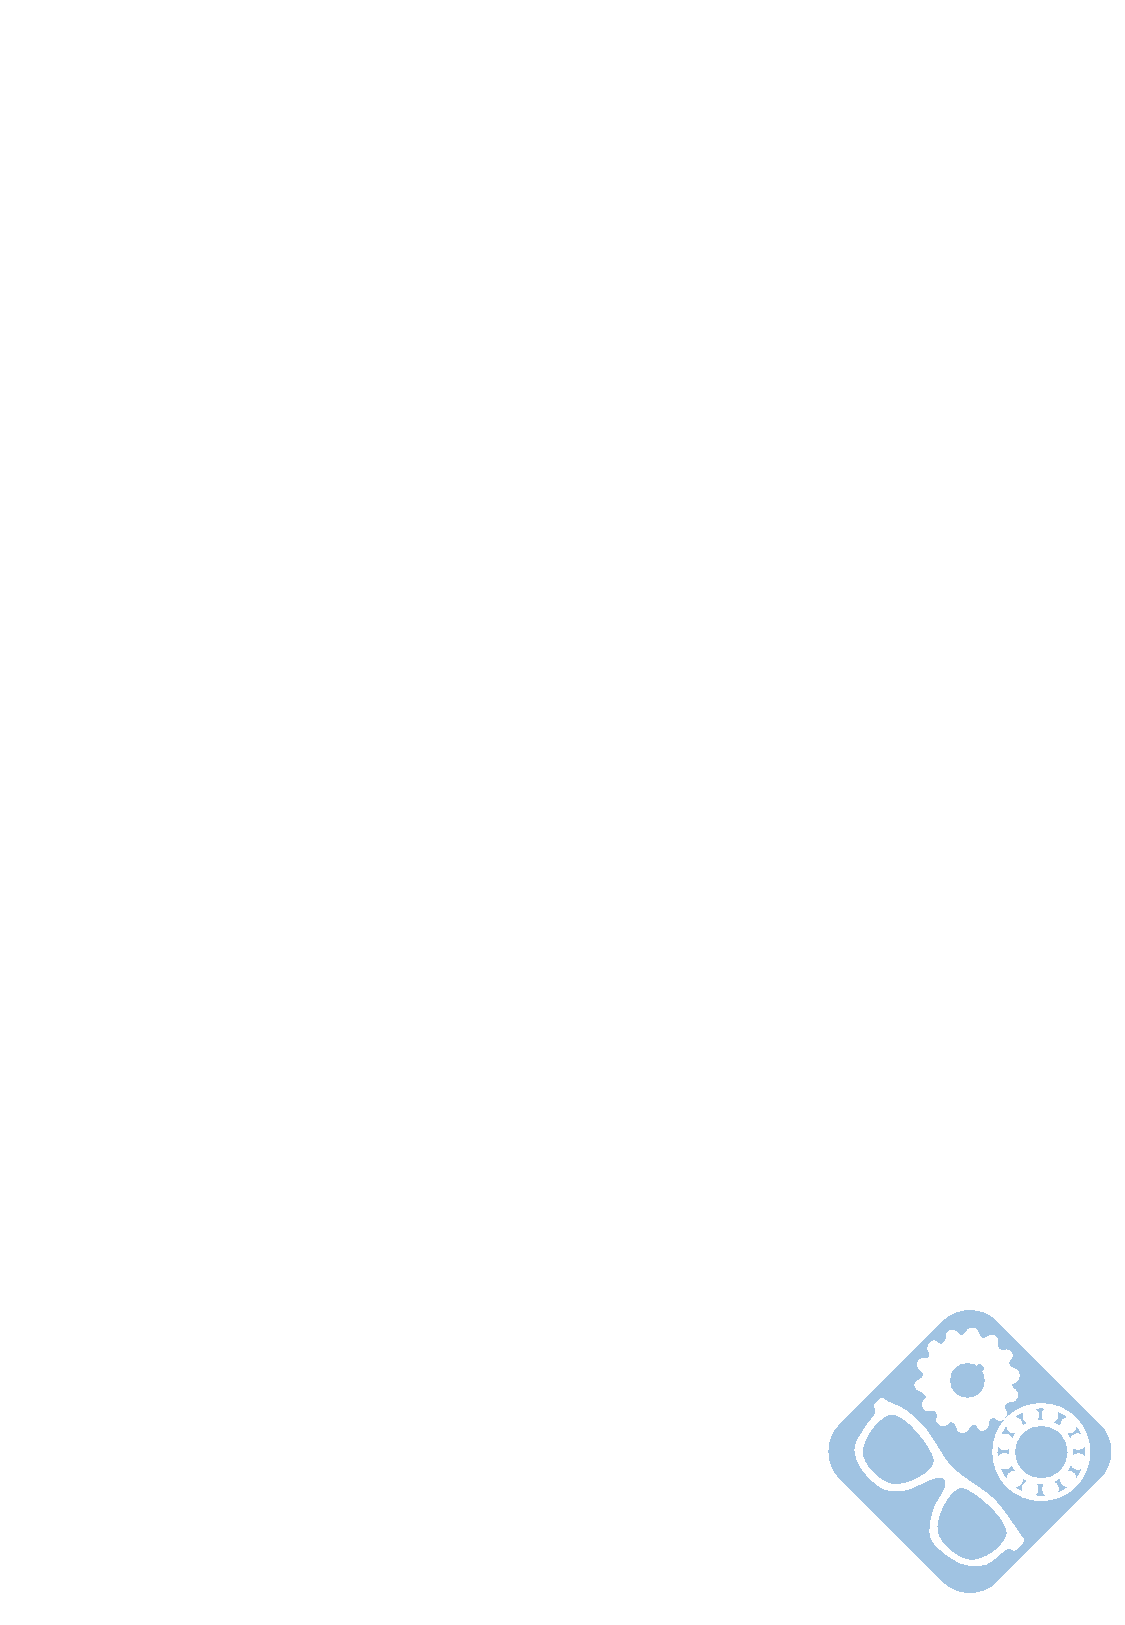
\includegraphics[width=\paperwidth,height=\paperheight,%
keepaspectratio]{../../img/fond4}%
\end{center}
\vfill
}}}

\begin{document}

\pagestyle{empty}

\vspace*{-3\baselineskip}

\AddToShipoutPicture*{\BackgroundPic}

\ifdef{\auteurdeux}{\begin{tabular}{>{\columncolor{gray!00}}m{.3\linewidth} m{.3\linewidth} >{\columncolor{gray!00}}m{.3\linewidth}}
Séquence : \sequence &  \multirow{3}{*}{\hspace{1cm}
\includegraphics[height=1.5cm]{../../img/logo}} &  \begin{flushright} \multirow{4}{*}{\hspace{1cm}
\includegraphics[height=4cm]{img/qrcode}}\end{flushright}\\
Document : \type\num \\
 \institute \\
 \auteurun\\
 \auteurdeux
\end{tabular}}{\begin{tabular}{>{\columncolor{gray!00}}m{.3\linewidth} m{.3\linewidth} >{\columncolor{gray!00}}m{.3\linewidth}}
Séquence : \sequence &  \multirow{3}{*}{\hspace{1cm}
\includegraphics[height=1.5cm]{../../img/logo}} &  \begin{flushright} \multirow{4}{*}{\hspace{1cm}
\includegraphics[height=4cm]{img/qrcode}}\end{flushright}\\
Document : \type\num \\
 \institute \\
 \auteurun
\end{tabular}}

\vspace{1cm}

\ifdef{\prive}{\begin{center}\colorbox{danger}{\Huge{Avec Correction}}\end{center}}{}

\begin{center}\huge{\nom}\end{center}

\vspace{2cm}

\ifdef{\imagedeux}{\begin{minipage}{0.49\linewidth}}{}
\begin{center}\includegraphics[height=5cm]{/home/renaud/Documents/Renaud/GitHub/django_education/systemes/\imageun}\end{center}
\ifdef{\imagedeux}{\end{minipage}\hfill
\begin{minipage}{0.49\linewidth}
\begin{center}\includegraphics[height=5cm]{/home/renaud/Documents/Renaud/GitHub/django_education/systemes/\imagedeux}\end{center}
\end{minipage}}{}

\vspace{5cm}


\begin{tabular}{p{.15\linewidth} >{\columncolor{white}}p{.8\linewidth}}
    \rowcolor{gray!20}
    Référence & S\sequence\ - \type\num \\
    Compétences & \competences \\
 	\rowcolor{gray!20}
    Description & \descrip \\
    Système & \systemes
  \end{tabular}

\newpage

\AddToShipoutPicture{\BackgroundPicdeux}

\pagestyle{normal}

\section{Trombone à coulisse}

\begin{figure}[htbp]
\begin{minipage}{0.49\linewidth}
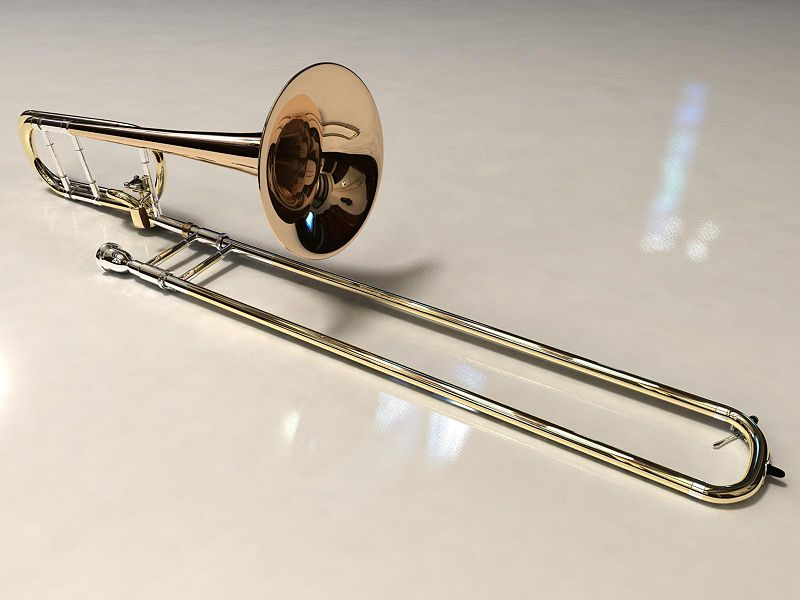
\includegraphics[width=0.9\linewidth]{img/Trombone}
\end{minipage}
\hfill
\begin{minipage}{0.48\linewidth}
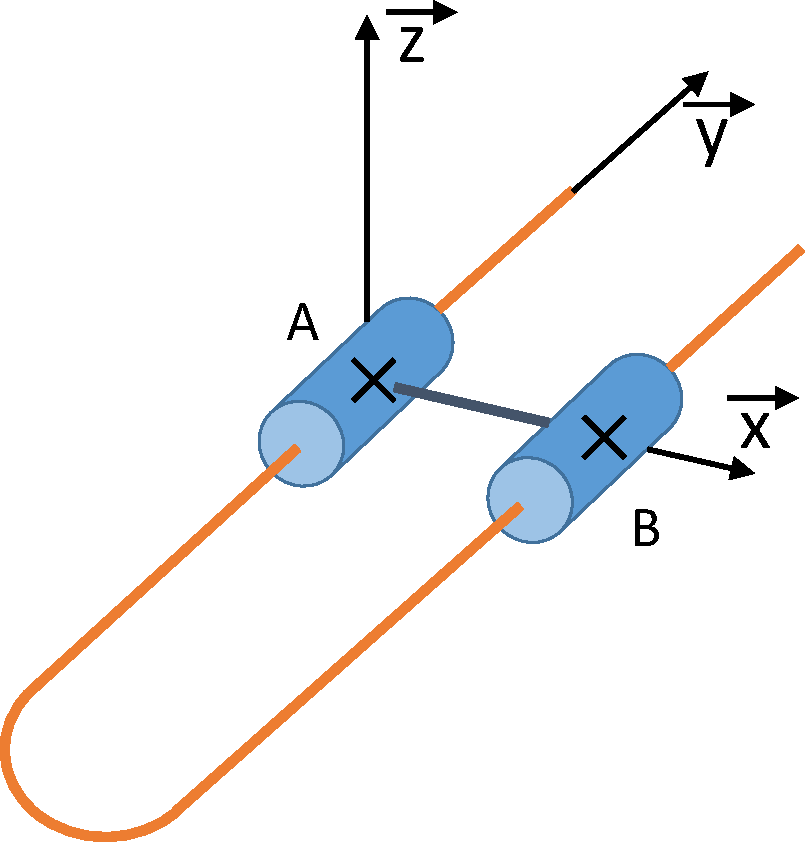
\includegraphics[width=0.9\linewidth]{img/Trombone_cin}
\end{minipage}
\end{figure}

Le \textbf{trombone} est un instrument de musique à vent et à embouchure de la famille des cuivres clairs. Le terme désigne implicitement le \textbf{trombone à coulisse} caractérisé par l'utilisation d'une \textbf{coulisse télescopique}, mais il existe également des modèles de trombone à pistons. Le trombone à coulisse est l'un des rares instruments à vent dont la maîtrise ne nécessite pas l'utilisation individuelle des doigts.

Le trombone est constitué d'un corps (0) et d'une coulisse (1). Le vecteur $\overrightarrow{AB}=e.\overrightarrow{x}$.

\paragraph{Question 1:} Écrire le graphe des liaisons du trombone à coulisse.

\paragraph{Question 2:} Écrire les torseurs cinématiques de chacune des liaisons et les déplacer au même point.

\paragraph{Question 3:} En déduire la liaison équivalente entre le \textbf{corps} du trombone et la \textbf{coulisse}.

\newpage

\section{Robot soudeur}

\begin{figure}[htbp]
\begin{minipage}{0.4\linewidth}
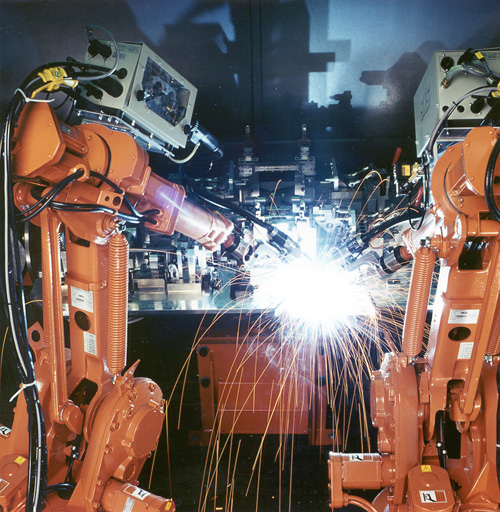
\includegraphics[width=0.9\linewidth]{img/robot_soudage}
\end{minipage}
\hfill
\begin{minipage}{0.55\linewidth}
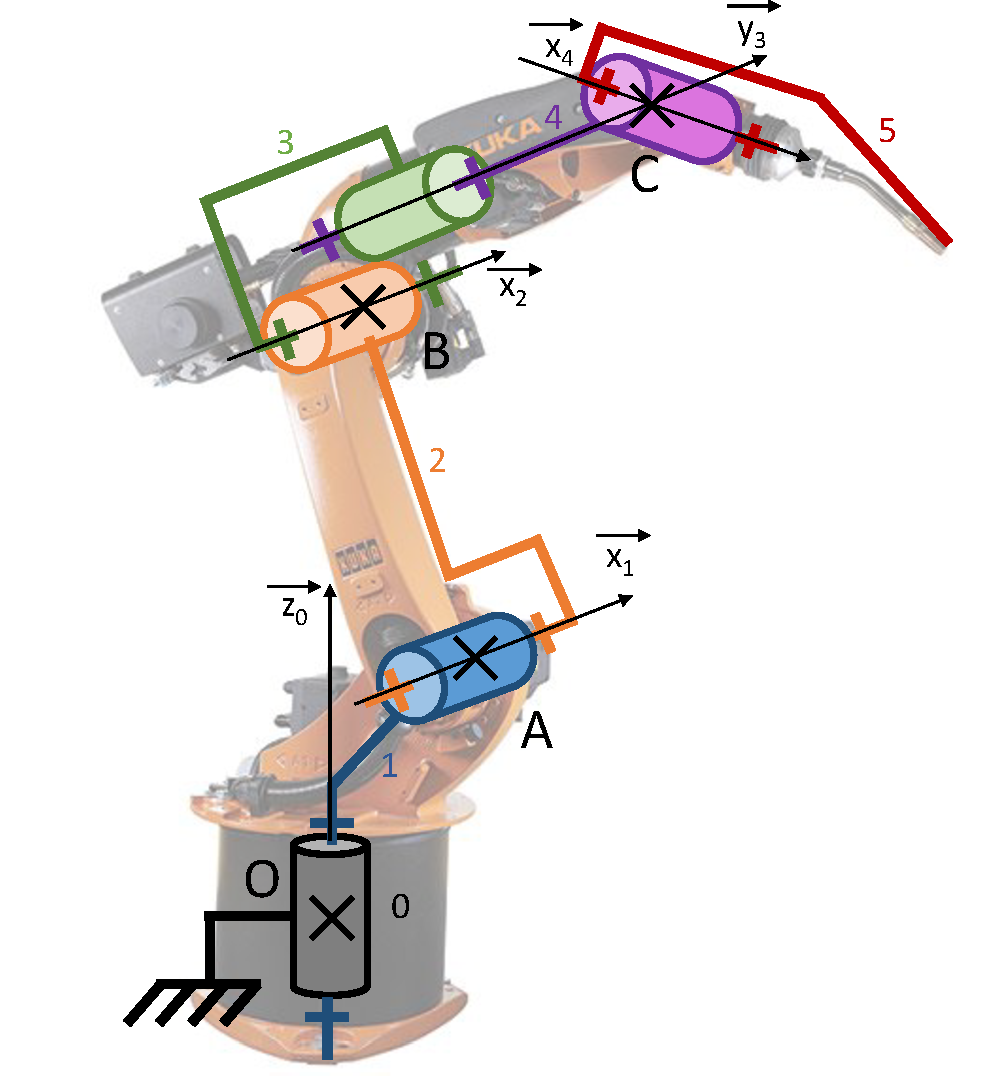
\includegraphics[width=0.9\linewidth]{img/Robot_cin}
\end{minipage}
\end{figure}

Un \textbf{robot industriel} est un système polyariticulé, à l'image d'un bras humain, composé de plusieurs degrés de liberté, permettant de déplacer et d'orienter un outil (organe effecteur) dans un espace de travail donné.

Il existe :
\begin{itemize}
 \item des robots de peinture ou de soudure largement utilisés dans l'industrie automobile,
 \item des robots de montage de dimension souvent plus réduite,
 \item des robots mobiles destinés à l'inspection souvent associés à de l'intelligence artificielle et capables, dans certains cas, de prendre en compte l'environnement.
\end{itemize}

Données:
\begin{itemize}
 \item $\overrightarrow{OA}=a.\overrightarrow{y_1}+b.\overrightarrow{z_1}$,
 \item $\overrightarrow{AB}=c.\overrightarrow{y_2}$,
 \item $\overrightarrow{BC}=d.\overrightarrow{y_3}+e.\overrightarrow{z_3}$.
\end{itemize}

\paragraph{Question 1:} Écrire le graphe des liaisons du robot soudeur.

\paragraph{Question 2:} Écrire les torseurs cinématiques des liaisons $\left\{V_{1/0}\right\}$ et $\left\{V_{2/1}\right\}$ et les déplacer au point O.

\paragraph{Question 3:} En déduire le torseur et le nombre de mobilité de la liaison équivalente entre la pièce $\textbf{2}$ et le \textbf{bâti}.

\paragraph{Question 4:} Écrire le torseur cinématique de la liaison $\left\{V_{3/2}\right\}$ et le déplacer au point O.

\paragraph{Question 5:} En déduire le torseur et le nombre de mobilité de la liaison équivalente entre la pièce $\textbf{3}$ et le \textbf{bâti}.

\paragraph{Question 6:} Écrire le torseur cinématique de la liaison $\left\{V_{4/3}\right\}$ et le déplacer au point O.

\paragraph{Question 7:} En déduire le torseur et le nombre de mobilité de la liaison équivalente entre la pièce $\textbf{4}$ et le \textbf{bâti}.\\

\paragraph{Question 8:} Conclure quant à l'intérêt d'ajouter des liaisons à une mobilité sur un bras robotisé.

\newpage

\section{Barrière sympact}

La cinématique de la transformation du mouvement de la barrière Sympact est présentée sur le schéma suivant.

\begin{center}
 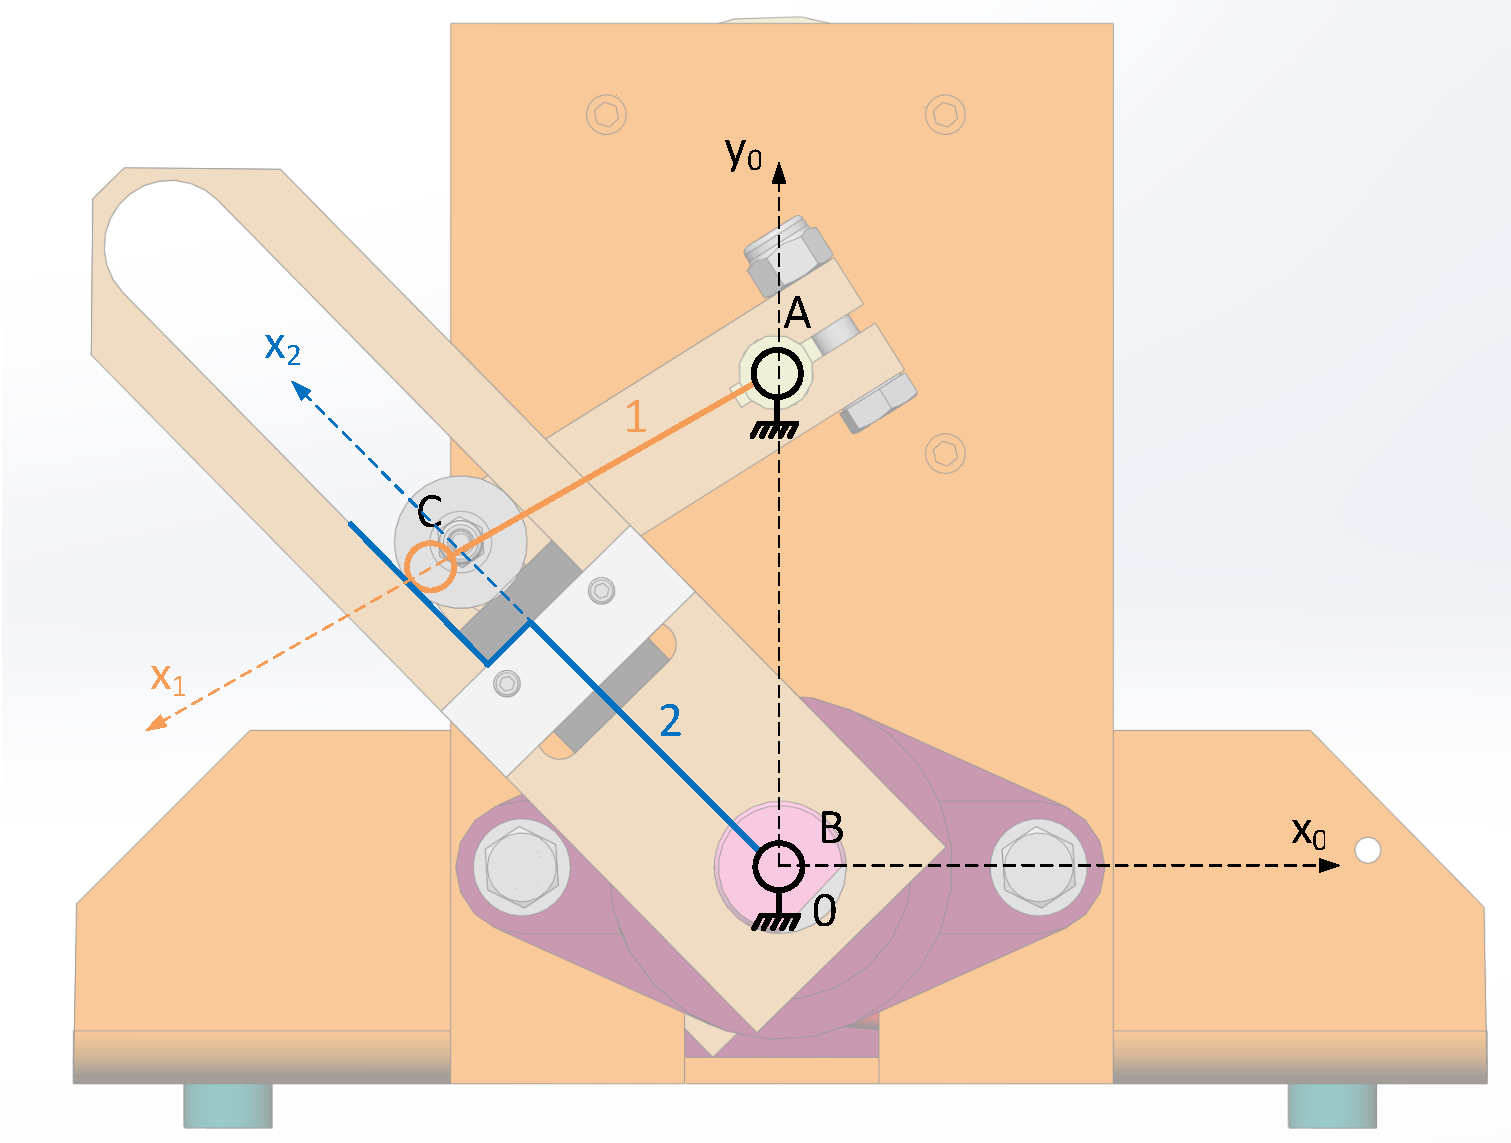
\includegraphics[width=0.8\linewidth]{img/Sympact_cin}
\end{center}

On donne les éléments géométriques suivants:
\begin{itemize}
 \item $\overrightarrow{AB}=-l_1.\overrightarrow{y_0}$,
 \item $\overrightarrow{AC}=l_2.\overrightarrow{x_1}$,
 \item $\theta_1=(\overrightarrow{x_0},\overrightarrow{x_1})=(\overrightarrow{y_0},\overrightarrow{y_1})$,
 \item $\theta_2=(\overrightarrow{x_0},\overrightarrow{x_2})=(\overrightarrow{y_0},\overrightarrow{y_2})$.
\end{itemize}

\paragraph{Question 1:} Déterminer les torseurs des liaisons suivantes $\left\{V_{1/0}\right\}$, $\left\{V_{2/0}\right\}$ et $\left\{V_{2/1}\right\}$.

\paragraph{Question 2:} Déplacer ces torseurs au point A, dans le repère $R_0$.

\paragraph{Question 3:} Déterminer la liaison équivalente $\left\{Ve_{2/0}\right\}$.

\paragraph{Question 4:} Déterminer le nombre de mobilités du système.

\ifdef{\public}{\end{document}}{}

\newpage

\pagestyle{correction}

\section{Correction}

\subsection{Trombone à coulisse}

\paragraph{Question 1:} Il y a deux liaisons entre le corps \textbf{0} et la coulisse \textbf{1}:
\begin{itemize}
 \item Pivot-glissant (A,$\overrightarrow{y}$),
 \item Pivot-glissant (B,$\overrightarrow{y}$).
\end{itemize}

\paragraph{Question 2:} ~\ \\

$\left\{V'_{1/0}\right\}=\left\{\begin{array}{c c} 0 & 0\\ \omega'_{10} & V'_{A,10} \\ 0 & 0
\end{array} \right\}_A$,
$\left\{V''_{1/0}\right\}=\left\{\begin{array}{c c} 0 & 0\\ \omega''_{10} & V''_{B,10} \\ 0 & 0 \end{array} \right\}_B$

$\overrightarrow{V_{A\in1/0}}=\overrightarrow{V_{B\in1/0}}+\overrightarrow{AB}\wedge \Omega_{1/0}=\begin{array}{c} 0 \\ V''_{B,10} \\ 0 \end{array}+\begin{array}{c} e\\ 0 \\ 0 \end{array} \wedge \begin{array}{c} 0\\ \omega''_{10} \\ 0 \end{array}$

$\left\{V''_{1/0}\right\}=\left\{\begin{array}{c c} 0 & 0\\ \omega''_{10} & V''_{B,10} \\ 0 & e.\omega''_{10} \end{array} \right\}_A$

$\left\{Ve_{1/0}\right\}=\left\{\begin{array}{c c} 0 & 0\\ \omega'_{10} & V'_{A,10} \\ 0 & 0
\end{array} \right\}_A=\left\{\begin{array}{c c} 0 & 0\\ \omega''_{10} & V''_{B,10} \\ 0 & e.\omega''_{10} \end{array} \right\}_A=\left\{\begin{array}{c c} 0 & 0 \\ 0 & V_{A,10} \\ 0 & 0 \end{array} \right\}_A$

\paragraph{Question 3:} La liaison équivalente est une glissière.

\subsection{Robot soudeur}

\paragraph{Question 1:} Les liaisons sont les suivantes:
\begin{enumerate}
 \item Pivot entre 0 et 1 (O,$\overrightarrow{z_0}$),
 \item Pivot entre 1 et 2 (A,$\overrightarrow{x_1}$),
 \item Pivot entre 2 et 3 (B,$\overrightarrow{x_2}$),
 \item Pivot entre 3 et 4 (C,$\overrightarrow{y_3}$),
 \item Pivot entre 4 et 5 (C,$\overrightarrow{x_4}$).
\end{enumerate}

\paragraph{Question 2:} ~\ \\
 
$\left\{V_{1/0}\right\}=\left\{\begin{array}{c c} 0 & 0\\ 0 &  \\ \omega_{10} & 0 \end{array} \right\}_{(O,R_0\ ou\ R_1)}$,
$\left\{V_{2/1}\right\}=\left\{\begin{array}{c c} \omega_{21} & 0\\ 0 & 0 \\ 0 & 0 \end{array} \right\}_{(A,R_1)}$.

$\overrightarrow{V_{O\in2/1}}=\overrightarrow{V_{A\in2/1}}+\overrightarrow{OA}\wedge \Omega_{2/1}=\left(\begin{array}{c} 0 \\ 0 \\ 0 \end{array}\right)+\left(\begin{array}{c} 0 \\ a \\ b \end{array}\right) \wedge \left(\begin{array}{c} \omega_{21} \\ 0 \\ 0 \end{array}\right)$

$\left\{V_{2/1}\right\}=\left\{\begin{array}{c c} \omega_{21} & 0\\ 0 & b.\omega_{21} \\ 0 & -a.\omega_{21} \end{array} \right\}_{(O,R_1)}$

\paragraph{Question 3:} ~\ \\

$\left\{V_{2/0}\right\}=\left\{\begin{array}{c c} \omega_{21} & 0\\ 0 & b.\omega_{21} \\ \omega_{10} & -a.\omega_{21} \end{array} \right\}_{(O,R_1)}$.

Il y a deux mobilités: $\omega_{10}$ et $\omega_{21}$.

\paragraph{Question 4:} ~\ \\

$\left\{V_{3/2}\right\}=\left\{\begin{array}{c c} \omega_{32} & 0\\ 0 & 0 \\ 0 & 0 \end{array} \right\}_{(B,R_1)}=\left\{\begin{array}{c c} \omega_{32} & 0\\ 0 & (b+c.sin\theta_{21}).\omega_{32} \\ 0 & -(a+c.cos\theta_{21}).\omega_{32} \end{array} \right\}_{(O,R_1)}$

\paragraph{Question 5:} ~\ \\

$\left\{V_{3/0}\right\}=\left\{\begin{array}{c c} \omega_{32}+\omega_{21} & 0\\ 0 & b.\omega_{21}+(b+c.sin\theta_{21}).\omega_{32} \\ \omega_{10} & -a.\omega_{21}-(a+c.cos\theta_{21}).\omega_{32} \end{array} \right\}_{(O,R_1)}$

Il y a trois mobilités: $\omega_{10}$, $\omega_{21}$ et $\omega_{32}$.


\paragraph{Question 6:} ~\ \\

$\left\{V_{4/3}\right\}=\left\{\begin{array}{c c} 0 & 0\\ \omega_{43} & 0 \\ 0 & 0 \end{array} \right\}_{(C,R_3)}$

$\overrightarrow{OC}=a.\overrightarrow{y_1}+b.\overrightarrow{z_1}+c.\overrightarrow{y_2}+d.\overrightarrow{y_3}+e.\overrightarrow{z_3}=a.\overrightarrow{y_1}+b.\overrightarrow{z_1}+c.\overrightarrow{y_2}+(d.cos \theta_{32}-e.sin \theta_{32}).\overrightarrow{y_2}+(d.sin \theta_{32}+e.cos \theta_{32}).\overrightarrow{z_2}$

$\overrightarrow{OC}=\left[a+c.cos \theta_{21}+d.cos (\theta_{32}+\theta_{21})-e.sin (\theta_{32}+\theta_{21})\right].\overrightarrow{y_1}$\\
$+\left[b+c.sin \theta_{21}+d.sin (\theta_{32}+\theta_{21})+e.cos (\theta_{32}+\theta_{21})\right].\overrightarrow{z_1}$

$\overrightarrow{\Omega_{4/3}}=\omega_{43}.\overrightarrow{y_3}=\omega_{43}.\left[cos(\theta_{32}+\theta_{21}).\overrightarrow{y_1}+sin(\theta_{32}+\theta_{21}).\overrightarrow{z_1}\right]$

$\overrightarrow{V_{O\in4/3}}=\left[\left[a+c.cos \theta_{21}+d.cos (\theta_{32}+\theta_{21})-e.sin (\theta_{32}+\theta_{21})\right].sin (\theta_{32}+\theta_{21})\right.$\\$\left.-\left[b+c.sin \theta_{21}+d.sin (\theta_{32}+\theta_{21})+e.cos (\theta_{32}+\theta_{21})\right].cos (\theta_{32}+\theta_{21})\right].\omega_{43}.\overrightarrow{x_1}$

En simplifiant, grâce aux formules trigonométriques, on obtient:
$\overrightarrow{V_{O\in4/3}}=\left[a.sin (\theta_{32}+\theta_{21})-b.cos (\theta_{32}+\theta_{21})+c.sin (\theta_{32})-e\right].\omega_{43}.\overrightarrow{x_1}$

Ce résultat aurait pu être trouvé directement en faisant le maximum de calculs dans le repère $R_3$.

$\overrightarrow{V_{O\in4/3}}=\overrightarrow{OC}\wedge\overrightarrow{\Omega_{4/3}}$

$\overrightarrow{V_{O\in4/3}}=(-a.sin(\theta_{32}+\theta_{21})+b.cos(\theta_{32}+\theta_{21})-c.sin(\theta_{32})+e).\overrightarrow{z_3}\wedge\omega_{4/3}.\overrightarrow{y_3}$

$\overrightarrow{V_{O\in4/3}}=(a.sin(\theta_{32}+\theta_{21})-b.cos(\theta_{32}+\theta_{21})+c.sin(\theta_{32})-e).\omega_{4/3}.\overrightarrow{x_3}$, avec $\overrightarrow{x_3}=\overrightarrow{x_1}$,donc:

$\overrightarrow{V_{O\in4/3}}=(a.sin(\theta_{32}+\theta_{21})-b.cos(\theta_{32}+\theta_{21})+c.sin(\theta_{32})-e).\omega_{4/3}.\overrightarrow{x_1}$.

On retrouve bien le résultat précédent.



\paragraph{Question 7:} ~\ \\

$\overrightarrow{\Omega_{4/0}}=(\omega_{32}+\omega_{21}).\overrightarrow{x_1}+\omega_{10}.\overrightarrow{z_1}+\omega_{43}.\left[cos(\theta_{32}+\theta_{21}).\overrightarrow{y_1}+sin(\theta_{32}+\theta_{21}).\overrightarrow{z_1}\right]$

$\overrightarrow{V_{O\in4/0}}=\left[\left[a+c.cos \theta_{21}+d.cos (\theta_{32}+\theta_{21})-e.sin (\theta_{32}+\theta_{21})\right].sin (\theta_{32}+\theta_{21})\right.$\\$\left.-\left[b+c.sin \theta_{21}+d.sin (\theta_{32}+\theta_{21})+e.cos (\theta_{32}+\theta_{21})\right].cos (\theta_{32}+\theta_{21})\right].\omega_{43}.\overrightarrow{x_1}$\\$+(b.\omega_{21}+(b+c.sin\theta_{21}).\omega_{32}).\overrightarrow{y_1}-(a.\omega_{21}+(a+c.cos\theta_{21}).\omega_{32}).\overrightarrow{z_1}$

$\left\{V_{4/0}\right\}=\left\{\begin{array}{c} 
\overrightarrow{\Omega_{4/0}} \\
\overrightarrow{V_{O\in4/0}}
\end{array} \right\}_{(O,R_1)}$. Il y a quatre mobilités: $\omega_{10}$, $\omega_{21}$ , $\omega_{32}$ et $\omega_{43}$.

%$\left\{V_{4/0}\right\}=$\\$\left\{\begin{array}{c c} \omega_{32}+\omega_{21} & \left[\left[a+c.cos \theta_{21}+d.cos (\theta_{32}+\theta_{21})-e.sin (\theta_{32}+\theta_{21})\right].sin (\theta_{32}+\theta_{21})\right.- \\ & \left.\left[b+c.sin \theta_{21}+d.sin (\theta_{32}+\theta_{21})+e.cos (\theta_{32}+\theta_{21})\right].cos (\theta_{32}+\theta_{21})\right].\omega_{43}\\ \omega_{43}.cos(\theta_{32}+\theta_{21}) & (b.\omega_{21}+(b+c.sin\theta_{21}).\omega_{32}) \\ \omega_{10}+\omega_{43}.sin(\theta_{32}+\theta_{21}) & -(a.\omega_{21}+(a+c.cos\theta_{21}).\omega_{32}) \end{array} \right\}_{(O,R_1)}$

\paragraph{Question 9:} A chaque liaison ajoutée une mobilité (une équation indépendante) est ajoutée. Celle-ci apparaît car les liaisons ajoutées sont des liaisons pivot (1ddl). Le système doit alors avoir 5 mobilités au total.

\subsection{Barrière Sympact}

\paragraph{Question 1:} ~\ \\

$\left\{V_{1/0}\right\}=\left\{\begin{array}{c c}
0 & 0 \\ 0 & 0 \\ \omega_{10} & 0 
\end{array}\right\}_A$,
$\left\{V_{2/0}\right\}=\left\{\begin{array}{c c}
0 & 0 \\ 0 & 0 \\ \omega_{20} & 0 
\end{array}\right\}_B$,
$\left\{V_{2/1}\right\}=\left\{\begin{array}{c c}
\omega_{x21} & V_{x21} \\ \omega_{y21} & 0 \\ \omega_{z21} & V_{z21} 
\end{array}\right\}_{C,R_2}$.

\paragraph{Question 2:} ~\ \\

$\left\{V_{1/0}\right\}=\left\{\begin{array}{c c}
0 & 0 \\ 0 & 0 \\ \omega_{10} & 0 
\end{array}\right\}_A$,
$\left\{V_{2/0}\right\}=\left\{\begin{array}{c c}
0 & -l_1.\omega_{20} \\ 0 & 0 \\ \omega_{20} & 0 
\end{array}\right\}_A$.\\
$\overrightarrow{V_{A\in 2/1}}=\overrightarrow{V_{C\in 2/1}}+\overrightarrow{AC}\wedge \overrightarrow{\Omega_{2/1}}$\\
$\overrightarrow{V_{A\in 2/1}}=\left(\begin{array}{c}
V_{x21}.cos(\theta_2) \\ V_{x21}.sin(\theta_2) \\ V_{z21}
\end{array}\right)+\left(\begin{array}{c}
l_2.cos(\theta_1) \\ l_2.sin(\theta_1) \\ 0
\end{array}\right)\wedge \left(\begin{array}{c}
\omega_{x21}.cos(\theta_2)-\omega_{y21}.sin(\theta_2) \\ \omega_{x21}.sin(\theta_2)+\omega_{y21}.cos(\theta_2) \\ \omega_{z21}
\end{array}\right)$ \\
$\overrightarrow{V_{A\in 2/1}}=\left(\begin{array}{c}
V_{x21}.cos(\theta_2)+l_2.sin(\theta_1).\omega_{z21} \\ V_{x21}.sin(\theta_2)-l_2.cos(\theta_1).\omega_{z21} \\ V_{z21}+l_2.cos(\theta_1).\left(\omega_{x21}.sin(\theta_2)+\omega_{y21}.cos(\theta_2)\right)-l_2.sin(\theta_1).\left(\omega_{x21}.cos(\theta_2)-\omega_{y21}.sin(\theta_2)\right)
\end{array}\right)$.

\paragraph{Question 3:} ~\ \\ 

$\left\{Ve_{2/0}\right\}=\left\{V_{2/1}\right\}+\left\{V_{1/0}\right\}=\left\{V_{2/0}\right\}$

$\left\{\begin{array}{l}
\omega e_{x20}=\omega_{x21}.cos(\theta_2)-\omega_{y21}.sin(\theta_2)+0=0 \\
\omega e_{y20}=\omega_{x21}.sin(\theta_2)+\omega_{y21}.cos(\theta_2)+0=0 \\
\omega e_{z20}=\omega_{z21}+\omega_{10}=\omega_{20} \\
Ve_{x20}=V_{x21}.cos(\theta_2)+l_2.sin(\theta_1).\omega_{z21}+0=-l_1.\omega_{20} \\
Ve_{y20}=V_{x21}.sin(\theta_2)-l_2.cos(\theta_1).\omega_{z21}+0=0 \\
Ve_{z20}=V_{z21}+l_2.cos(\theta_1).\left(\omega_{x21}.sin(\theta_2)+\omega_{y21}.cos(\theta_2)\right)-l_2.sin(\theta_1).\left(\omega_{x21}.cos(\theta_2)-\omega_{y21}.sin(\theta_2)\right)+0=0 
\end{array}\right.$

Ainsi, $\omega_{x21}=\omega_{y21}=0$

$\left\{\begin{array}{l}
\omega e_{x20}=0 \\
\omega e_{y20}=0 \\
\omega e_{z20}=\omega_{z21}+\omega_{10}=\omega_{20} \\
Ve_{x20}=V_{x21}.cos(\theta_2)+l_2.sin(\theta_1).\omega_{z21}+0=-l_1.\omega_{20} \\
Ve_{y20}=V_{x21}.sin(\theta_2)-l_2.cos(\theta_1).\omega_{z21}+0=0 \\
Ve_{z20}=0 
\end{array}\right.$

\paragraph{Question 4:} ~\ \\

$\left\{\begin{array}{l}
\omega_{x21}.cos(\theta_2)-\omega_{y21}.sin(\theta_2)+0=0 \\
\omega_{x21}.sin(\theta_2)+\omega_{y21}.cos(\theta_2)+0=0 \\
\omega_{z21}+\omega_{10}=\omega_{20} \\
V_{x21}.cos(\theta_2)+l_2.sin(\theta_1).\omega_{z21}+0=-l_1.\omega_{20} \\
V_{x21}.sin(\theta_2)-l_2.cos(\theta_1).\omega_{z21}+0=0 \\
V_{z21}+l_2.cos(\theta_1).\left(\omega_{x21}.sin(\theta_2)+\omega_{y21}.cos(\theta_2)\right)-l_2.sin(\theta_1).\left(\omega_{x21}.cos(\theta_2)-\omega_{y21}.sin(\theta_2)\right)+0=0 
\end{array}\right.$

Étude du système:
\begin{itemize}
 \item 7 inconnues cinématiques: $\omega_{10}$, $\omega_{20}$, $\omega_{x21}$, $\omega_{y21}$,$\omega_{z21}$, $V_{x21}$ et $V_{z21}$,
 \item 6 équations indépendantes.
\end{itemize}

On en déduit: $m = I_C - Rg(E)=4-3=1$, le système possède 1 mobilité.

De plus, on remarque aussi dans ce cas que: $h=E-Rg(E)=6-6=0$, le modèles est isostatique.

\end{document}
